\PassOptionsToPackage{unicode=true}{hyperref} % options for packages loaded elsewhere
\PassOptionsToPackage{hyphens}{url}
%
\documentclass[]{article}
\usepackage{lmodern}
\usepackage{amssymb,amsmath}
\usepackage{ifxetex,ifluatex}
\usepackage{fixltx2e} % provides \textsubscript
\ifnum 0\ifxetex 1\fi\ifluatex 1\fi=0 % if pdftex
  \usepackage[T1]{fontenc}
  \usepackage[utf8]{inputenc}
  \usepackage{textcomp} % provides euro and other symbols
\else % if luatex or xelatex
  \usepackage{unicode-math}
  \defaultfontfeatures{Ligatures=TeX,Scale=MatchLowercase}
\fi
% use upquote if available, for straight quotes in verbatim environments
\IfFileExists{upquote.sty}{\usepackage{upquote}}{}
% use microtype if available
\IfFileExists{microtype.sty}{%
\usepackage[]{microtype}
\UseMicrotypeSet[protrusion]{basicmath} % disable protrusion for tt fonts
}{}
\IfFileExists{parskip.sty}{%
\usepackage{parskip}
}{% else
\setlength{\parindent}{0pt}
\setlength{\parskip}{6pt plus 2pt minus 1pt}
}
\usepackage{hyperref}
\hypersetup{
            pdftitle={Draft Report},
            pdfauthor={Ngoc Duong, Cui Sitong (sc4636), Xinru Wang(xw2676), Jin Ge},
            pdfborder={0 0 0},
            breaklinks=true}
\urlstyle{same}  % don't use monospace font for urls
\usepackage[margin=1in]{geometry}
\usepackage{graphicx,grffile}
\makeatletter
\def\maxwidth{\ifdim\Gin@nat@width>\linewidth\linewidth\else\Gin@nat@width\fi}
\def\maxheight{\ifdim\Gin@nat@height>\textheight\textheight\else\Gin@nat@height\fi}
\makeatother
% Scale images if necessary, so that they will not overflow the page
% margins by default, and it is still possible to overwrite the defaults
% using explicit options in \includegraphics[width, height, ...]{}
\setkeys{Gin}{width=\maxwidth,height=\maxheight,keepaspectratio}
\setlength{\emergencystretch}{3em}  % prevent overfull lines
\providecommand{\tightlist}{%
  \setlength{\itemsep}{0pt}\setlength{\parskip}{0pt}}
\setcounter{secnumdepth}{0}
% Redefines (sub)paragraphs to behave more like sections
\ifx\paragraph\undefined\else
\let\oldparagraph\paragraph
\renewcommand{\paragraph}[1]{\oldparagraph{#1}\mbox{}}
\fi
\ifx\subparagraph\undefined\else
\let\oldsubparagraph\subparagraph
\renewcommand{\subparagraph}[1]{\oldsubparagraph{#1}\mbox{}}
\fi

% set default figure placement to htbp
\makeatletter
\def\fps@figure{htbp}
\makeatother


\title{Draft Report}
\author{Ngoc Duong, Cui Sitong (sc4636), Xinru Wang(xw2676), Jin Ge}
\date{4/15/2020}

\begin{document}
\maketitle

\hypertarget{objective}{%
\subsection{Objective}\label{objective}}

Breast cancer is one of the most common cancers in women. However, early
diagnoses of breast cancer can aid in reducing the mortatlity rate.
Additionally, advances in imaging technologies and statistical
methodologies have allowed for higher-quality data and novel models that
could improve the precision of breast cancer diagnoses. The purpose of
our project is to build and compare different models in classifying
breast cancer tumor as benignant or malignant based on image-based
predictors. Specifically, we are look to build a logistic regression
model using Newton-Raphson method, and a logistic-LASSO model using
coordinate-wise optimization algorithm.

\hypertarget{dataset}{%
\subsubsection{Dataset}\label{dataset}}

There were 569 images collected independently from patients, 212 of whom
had malignant tumor and 357 were benign cases. The images were broken
down into 30 predictors, corresponding to the mean, standard deviation,
and largest values (points on the tails) of the following 10 features:

\begin{itemize}
\item radius (mean of distances from center to points on the perimeter)
\item texture (standard deviation of gray-scale values)
\item perimeter
\item area
\item smoothness (local variation in radius lengths)
\item compactness (perimeter\^ 2 / area - 1.0)
\item concavity (severity of concave portions of the contour)
\item concave points (number of concave portions of the contour)
\item symmetry
\item fractal dimension ("coastline approximation" - 1)
\end{itemize}

\hypertarget{data-cleaning}{%
\subsubsection{Data cleaning}\label{data-cleaning}}

As shown in the pairwise correlation plot (\textbf{Fig. 1}), we can
observe the presence of some strong multicollinearity among the
predictors. For instance, the radius\_mean variable has almost perfect
correlation of 1 and 0.99 with perimeter\_mean and area\_mean variables,
respectively. We then left out variables that are correlated by more
than 85\% with other predictors. The final dataset contained 13
predictors.

Next, considering the LASSO is not scale-invariant, we standardized the
design matrix. This is to ensure comparability of estimates by the
logistic-LASSO model and Newton-Raphson/logistic regression model. The
standardization formula is as follows:

\(standardized(x_{ij}) = \frac{x_{ij} - \bar{x_{j}}}{std(x_{j})}\) for
\(i = 1,2,...30\) and \(j = 1,2,..., 569\)

Finally, we recoded response variable such that ``malignancy'' = 1, and
``benign'' = 0.

\hypertarget{newton-raphson-model}{%
\paragraph{Newton-Raphson model}\label{newton-raphson-model}}

We used logistic regression to classify the malignancy of tissue.
Malignancy corresponds to response variable being 1 (\(y^{(i)} = 1\)).

Log likelihood is
\[l(y;\beta) = \sum^n_{i = 1} \{y_{(i)} log\mu_{(i)} + (1 - y_{(i)}) log(1 - \mu_{(i)})\}\]

Its gradient is given by
\[g: \bigtriangledown l(y;\beta) = \sum^n_{i = 1} (y_{(i)} - \mu_{(i)}) x_{(i)} = X^T(y - \mu)\]

Its Hessian matrix is given by
\[H: \bigtriangledown^2 l(y;\beta) = -\sum^n_{i = 1} \mu_{(i)} (1 - \mu_{(i)}) x_{(i)} (x_{(i)})^T = -X^TSX\]
where \(S = diag(\mu_{(i)} (1 - \mu_{(i)}))\), and
\[\mu_{(i)} = p_{\theta}(y = 1|x) = \frac{e^{X_{i}\beta}}{1+e^{X_{i}\beta}}\]

Since we have several predictors, we want to optimize several likehood
functions simultaneously. This is equivalent to solving a system of
log-likelihood equations \(\bigtriangledown l(y;\beta_{j}) = 0\) where
\(j = 1,2,...13\). To achieve this, we used the Newton Raphson
algorithm.

\hypertarget{newton-raphson-algorithm}{%
\paragraph{Newton-Raphson Algorithm}\label{newton-raphson-algorithm}}

Starting at a current point \(\beta_{i}\), we can expand the
log-likelihood function around this point using Taylor's expansion,
which gives a neighborhood of \(\beta_{i}\) containing \(\beta_{i+1}\)
which increases the likelihood. The equation below can be used to
iteratively update \(\beta_{i}\) until the sequence converges and
\(\bigtriangledown l(y;\beta_{j}) = 0\) is satisfied:

\(\beta_{i+1} = \beta_{i}- [\bigtriangledown^2 l(\beta_{i})]^{-1} \bigtriangledown l(\beta_{i})\).

\begin{itemize}
\tightlist
\item
  Modifications to Newton-Raphson
\end{itemize}

When implementing Newton-Raphson, we need to check at every step, that
the updating direction (for \(\beta_{i+1}\)) is heading to a maximum,
and that the point is moving sufficient distances towards the maximum so
we do not miss it. Therefore, we also implemented some modifications,
specifically gradient descent and step-halving.

\begin{itemize}
\tightlist
\item
  For step-halving, we modified the updating function for
  \(\beta_{i+1}\) as follows:
\end{itemize}

\(\beta_{i+1} = \beta_{i}-\lambda [\bigtriangledown^2 l(y;\beta_{i})]^{-1} \bigtriangledown l(y;\beta_{i})\),
where \(\lambda = 1\) until \(l(\beta_{i+1}) \leq l(\beta_{i})\), which
means the new point would have gone too far. Then, we can search for a
value \(\lambda\) such that
\(l(\beta_{i+1}, \lambda) \geq l(\beta_{i})\). At this step, we can cut
the step, or \(\lambda\) in half for each sub-iteration.

\begin{itemize}
\tightlist
\item
  For gradient descent, at every iteration, we checked whether
  \(\bigtriangledown^2 l(y;\beta)\) is negative definite (signifying the
  point is moving in the right direction). If
  \(\bigtriangledown^2 l(y;\beta)\) is not, we replace it with a similar
  negative definite matrix, such as
  \(\bigtriangledown^2 l(y;\beta) - \gamma I\) where \(\gamma\) is
  chosen such that the resulting matrix is negative definite. Naturally,
  this \(\gamma\) must be greater than any of the elements of the
  diagonal matrix \(D\) obtained by eigendecomposing
  \(\bigtriangledown^2 l(y;\beta) = P^{T}DP\).
\end{itemize}

\hypertarget{logistic-lasso-model}{%
\subsubsection{Logistic-LASSO model}\label{logistic-lasso-model}}

The LASSO method aims to minimizes the following equation with a penalty
term, a quardratic approximation to the negative log likelihood by
taylor expansion around the current estimate, which is:

\[
\begin{aligned}
f(\beta) = \frac{1}{2n}\Sigma^n_{i=1}w_{i}(z_{i}-\Sigma^p_{j=1}x_{i,j}\beta_{j})^2 + \lambda \Sigma^p_{j=1}|\beta_{j}|, \lambda \geq 0
\end{aligned}
\]

where

\begin{itemize}
\tightlist
\item
  \(w_{i}\) are the working weights, defined as
  \(\tilde{p}(x_i)(1-\tilde{p}(x_i))\), and \(p_{i}\) is the probability
  of event for each observation
\item
  \(z_i\) are the working response = \tilde{\beta}\_0+
  x\_i\^{}T\tilde{\beta} +
  \frac{y_i-\tilde{p}(x_i)}{\tilde{p}(x_i)(1-\tilde{p}(x_i))},
  \text{working response}\textbackslash{}
\end{itemize}

Then, each \(\beta_{i}\) is optimized using the folllowing equation:

\[
\begin{aligned}
\tilde\beta_{i} = \frac{S(\Sigma_{i}w_{i}x_{i,j}(y_{i}-\tilde{y}^{(-j)}_{i}),\lambda)}{\Sigma_{i}w_{i}x_{i,j}^2}
\end{aligned}
\]

where \(S(\hat\beta, \gamma)\) is called soft-threshold and is defined
as
\(S(\hat{\beta}, \lambda) = sign(\hat{\beta})(|\hat{\beta}| - \lambda)_{+}\)

Coordinate-wise Descent algorithm is used to minimize this function. We
can form a quardratic approximation to the negative log likelihood by
taylor expansion around the current estimate, which is:

\[
f(\beta) = -\frac{1}{2n}\sum_{i=1}^{n}w_i(z_{i} - \sum_{j=0}^{p}x_{i,j}\beta_{j})^{2} + C(\tilde{\beta})
\] where \[
\begin{aligned}
& z_i = \tilde{\beta}_0+ x_i^T\tilde{\beta} + \frac{y_i-\tilde{p}(x_i)}{\tilde{p}(x_i)(1-\tilde{p}(x_i))}, \text{working response}\\
& w_i = \tilde{p}(x_i)(1-\tilde{p}(x_i)), \text{working weights}
\end{aligned}
\] and \(\tilde{p}(x_i)\) is evaluated at the current parameters, the
last term is constant. The Newton update is obtained by minimizing the
\(f(\beta)\)

The coordinate descent algorithm to solve the penalized weighted least
squares problem
\[\max_{\beta \in \mathbb{R}^{p+1}} \{ f(\beta) + \lambda P(\beta)\}\]

\hypertarget{results}{%
\subsection{Results}\label{results}}

The coefficient estimates can be found in (\textbf{Table 1}).
Newton-Raphson algorithm gives quite similar estimates to those in the
logistic regression model produced by GLM package. For the
logistic-LASSO model, we can see the coefficient estimates are
approximately close to the ones produced by GLMnet with 5-fold
cross-validation. They do not exactly match, however, due to the
potential dissimilarities in set-up conditions in our implementation and
theirs.

The path of solution could be found in (\textbf{Figure 3}), and the
distribution of cross-validated MSEs produced by the hand-built
logistic-LASSO model could be found in (\textbf{Figure 4}). Five-fold
cross-validation suggested the best \(\lambda\) is 0.00454, which
corresponds to the lowest cross-validated MSE. A similar distribution of
cross-validated MSEs produced by the GLMNet package in R can be found in
(\textbf{Fig. 4}). Here, 5-fold cross-validation suggested the best
\(\lambda\) is 0.0037.

Lastly, we wanted to compare the prediction performance using MSE as a
criteria. We examined this undertwo scenarios, one is with 5-fold
cross-validation, and the other is 5-fold repeated cross-validation
(number of repeats is 5). These distributions can be found in Figure 3
and 4, respectively. We noticed that the cross-validated MSE of both
Newton Raphson and logistic-LASSO are similary distributed, although the
latter seems to perform slightly less well. On the other hand, GLMnet
gives the most consistently well performance. Nonetheless, the errors
were all in close proximity with one another so we are confident they
all very good discriminatory power.

\hypertarget{conclusions}{%
\subsubsection{Conclusions}\label{conclusions}}

The report aimed to explore how different models perform at the same
task of classifying breast cancer tumors into benign and malignant types
using various predictors derived from the tumor images. Since we have
eliminated most multicollinearity at the beginning, it is reasonable to
expect Newton-Raphson and logistic-LASSO to have quite similar
discriminatory performance. On the other hand, we would expect to see
logistic-LASSO to perform better than Newton Raphson in terms of
predictive ability in the presence of higher-dimensional data, and with
more correlated predictors. We will aim to explore this further as more
time and bandwidth allow. All in all, these models we looked at in this
report nevertheless perform decently in classifying correctly each type
of breast cancer.

\clearpage

\hypertarget{appendix}{%
\subsection{Appendix}\label{appendix}}

\hypertarget{figure}{%
\subsubsection{Figure}\label{figure}}

\begin{figure}[h]

{\centering 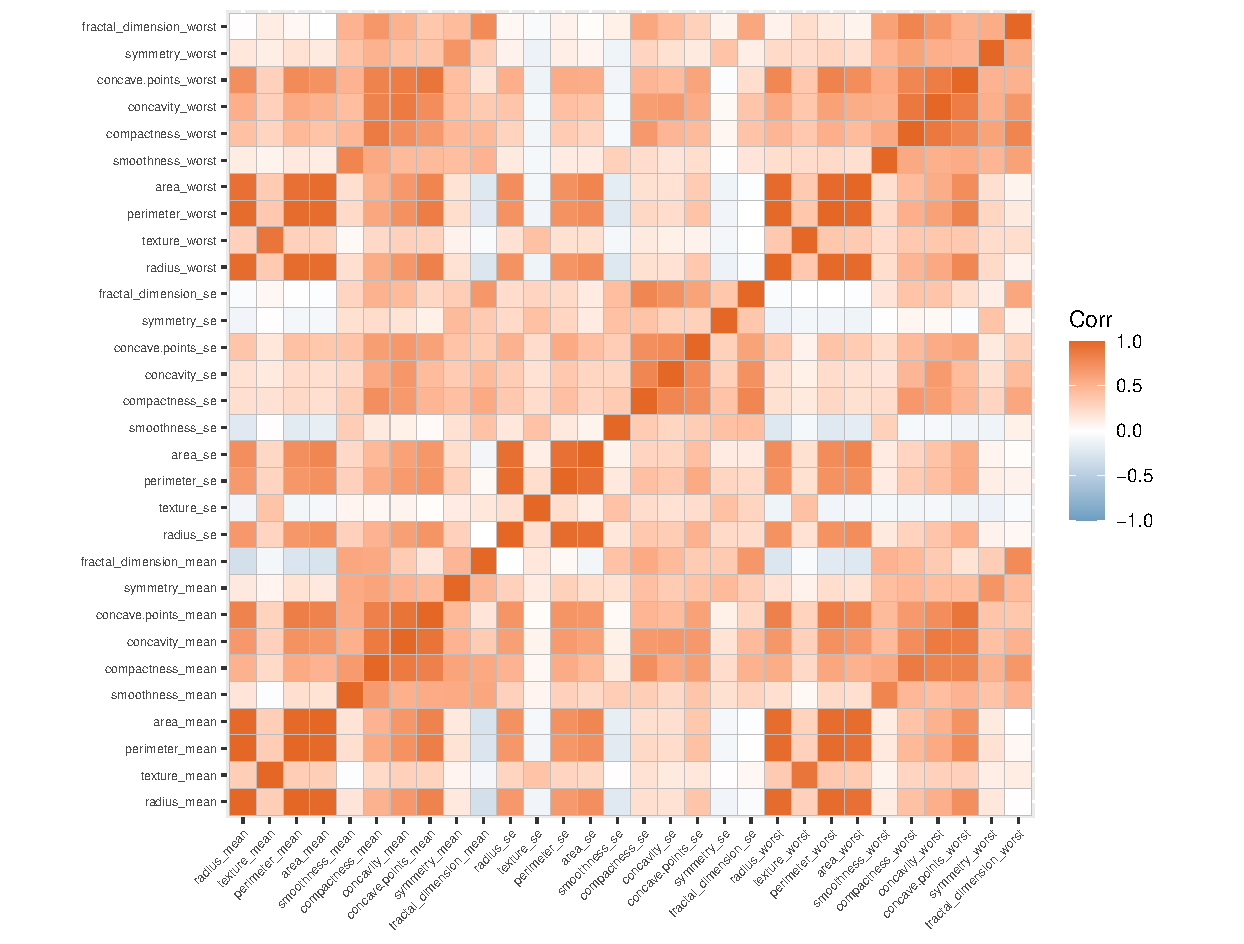
\includegraphics[width=0.8\linewidth]{plot1} 

}

\caption{Multicollinearity plot of the dataset}\label{fig:unnamed-chunk-1}
\end{figure}

\begin{figure}[h]

{\centering 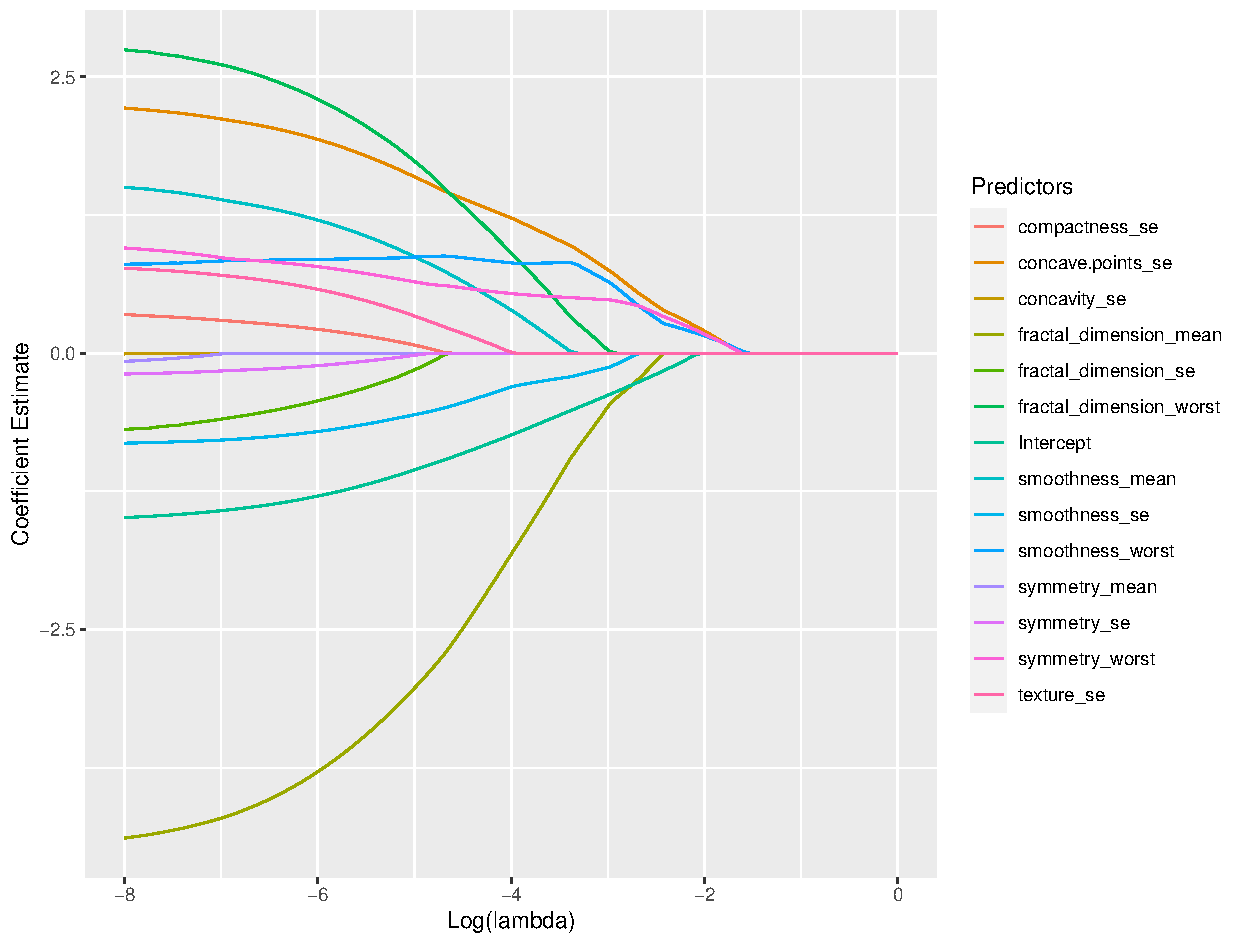
\includegraphics[width=0.7\linewidth]{plot2} 

}

\caption{The path of solution}\label{fig:unnamed-chunk-2}
\end{figure}

\begin{figure}[h]

{\centering 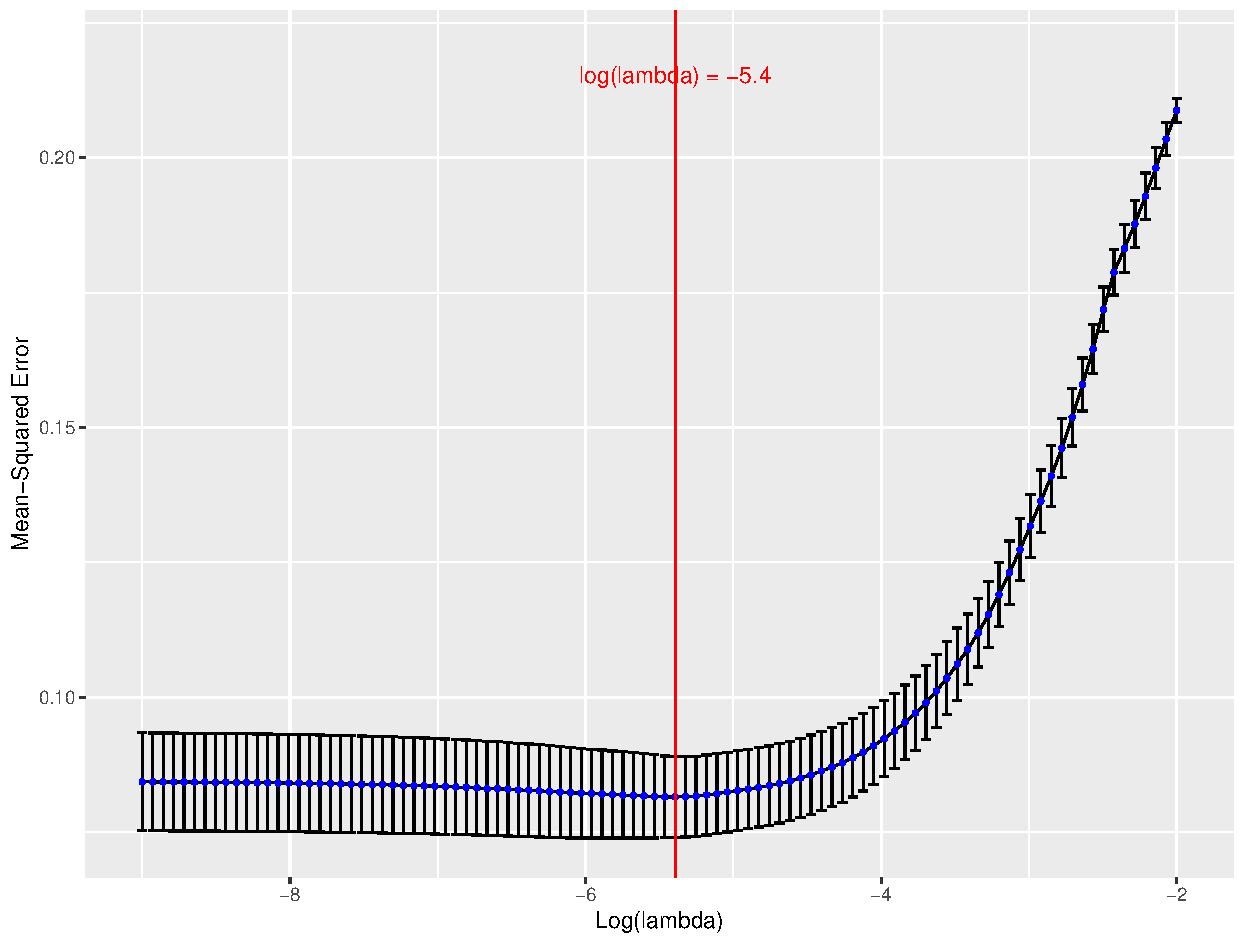
\includegraphics[width=0.8\linewidth]{plot3} 

}

\caption{Plot of cross-validated MSEs by hand-built model}\label{fig:unnamed-chunk-3}
\end{figure}

\begin{figure}[h]

{\centering 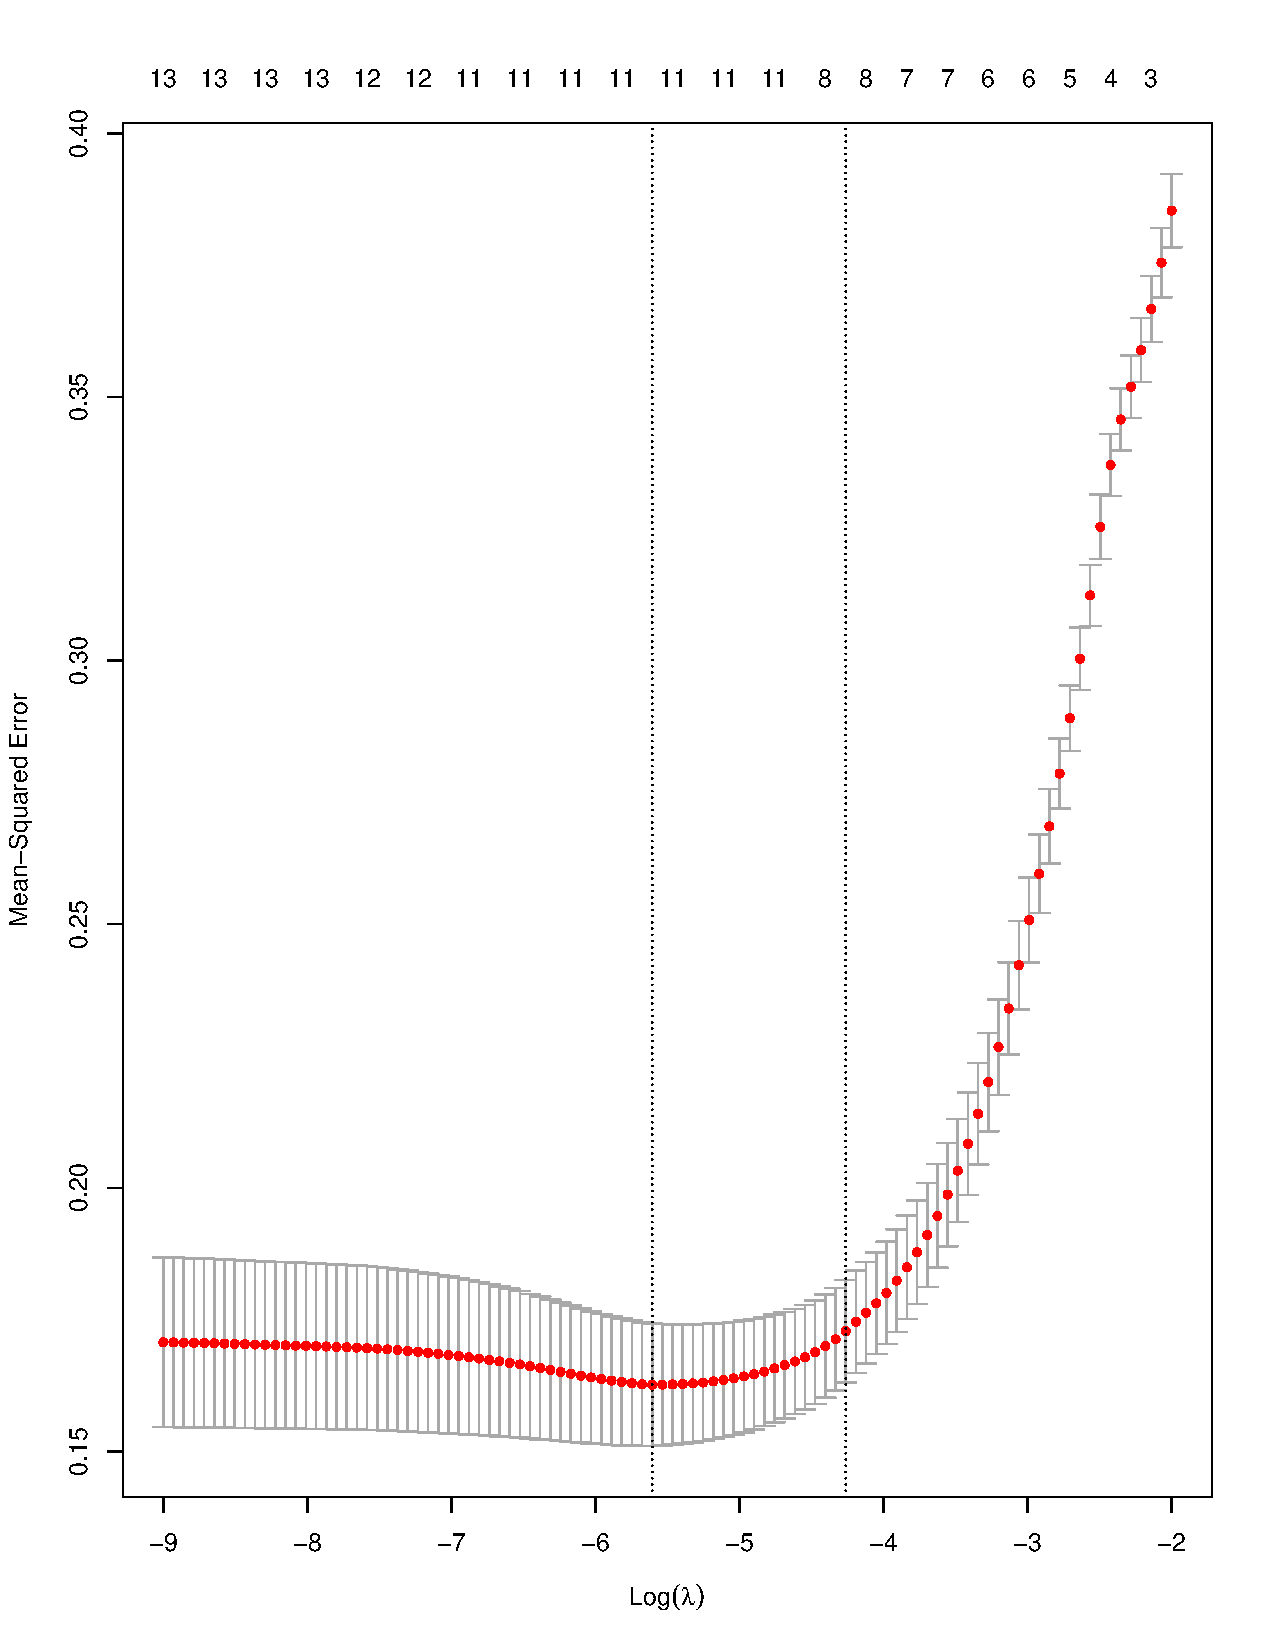
\includegraphics[width=0.6\linewidth]{plot4} 

}

\caption{Plot of cross-validated MSEs by the GLMNet}\label{fig:unnamed-chunk-4}
\end{figure}

\begin{figure}[h]

{\centering 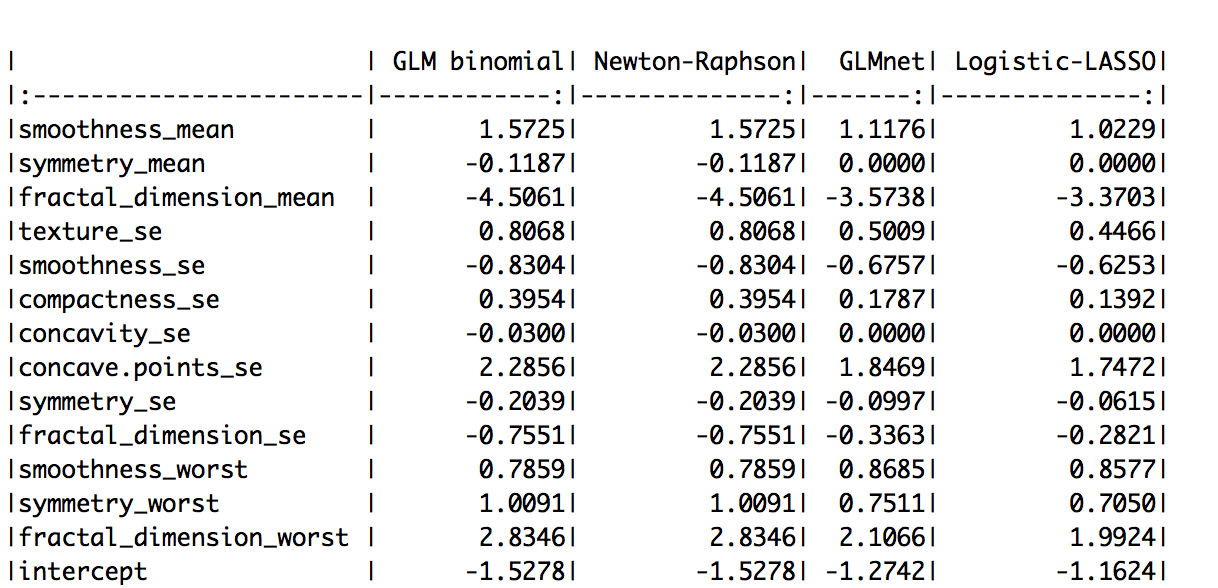
\includegraphics[width=0.8\linewidth]{table1} 

}

\caption{The coefficient estimates of each model}\label{fig:unnamed-chunk-5}
\end{figure}

\[
\begin{aligned}
& z_i = \tilde{\beta}_0+ x_i^T\tilde{\beta} + \frac{y_i-\tilde{p}(x_i)}{\tilde{p}(x_i)(1-\tilde{p}(x_i))}, \text{working response}\\
& w_i = \tilde{p}(x_i)(1-\tilde{p}(x_i)), \text{working weights}
\end{aligned}
\]

\end{document}
